\section{Requirements for Android application}

\subsection{Application features}\label{FeaturesSection}

\paragraph{Vehicle Routing Problem}
Standard OptaPlanner distribution \cite{OptaPlannerDistribution} contains demonstration examples. One of the examples is
Vehicle Routing application. Its source code already contains Vehicle Routing Problem model which should be included in
this application. Also it contains some tools for importing specific \texttt{.vrp} files. Graphical user interface
cannot be ported because application is written by Awt and Swing libraries which are not included in Android API as
described in Section \ref{OptaPlannerChapter}. Thanks to that and because it is good practise to adapt the application
to Android mobile platform, graphical user interface and functions of application should be completely rewritten and
adjusted to fulfill aspects of Android application development.

\paragraph{Application settings}
Application without any settings is too static and user cannot do much with it. Therefore, it should be option to choose
problem solving algorithm which can show that not all algorithms are suitable for such problems. Another option should
be setting of the time limit of caculation. Thanks to this, when process is terminated, last solution should remains
shown on the screen. It should be also possible to terminate process before time limit manually.

\paragraph{File opening}
Original Vehicle Routing application contains \texttt{.vrp} example files. These files should be compatible with created
application and some of them should be included. It should be possible to open these files and display them similar way
as in original application.

\paragraph{Solution diplaying}
When user selects file, unsolved solution should be displayable on the application screen. After start of solving
process, new best solution also should be displayable every time when new it is found. Application should further
contains resources how to display actual statistic information about solved problem.

\paragraph{License}
Whole application should be distributed as opensource software and it should be written under Apache License 2.0.
Source code must be publicly available on the internet to guide other persons how to use OptaPlaner in their projects.

\subsection{Android devices support}
Before the development starts, it is good to clarify for which version of Android will be application supported. Every
version of Android comes with new API and new functionality. Biggest changes comes when first number of version is
changed. Table \ref{distributon} shows actual distributions of Android verisons on devices.

Versions 2.x.x are on the decline, the most used versions are 4.x with higest percentage representation and the newest
version 5.x is not so much used yet but their participation grows. Therefore it was decided that application should
supports android from version 4.0 (API 14). It desides which resource can be used for application proposal and
development and how application should be tested.

\begin {table}[h!]
    \begin{tabular}{|c|c|r|}
        \hline
        Android version   & API   & Distribution  \\ \hline \hline
        2.2               & 8     & 0.4 \%        \\ \hline
        2.3.3 -- 2.3.7    & 10    & 6.4 \%        \\ \hline
        4.0.3 -- 4.0.4    & 15    & 5.7 \%        \\ \hline
        4.1               & 16    & 16.5 \%       \\ \hline
        4.2               & 17    & 18.6 \%       \\ \hline
        4.3               & 18    & 5.6 \%        \\ \hline
        4.4               & 19    & 41.4 \%       \\ \hline
        5.0               & 21    & 5.0 \%        \\ \hline
        5.1               & 22    & 0.4 \%        \\ \hline
    \end{tabular}
    \centering
    \caption{Android version distributon \cite{Dashboards}}
    \label{distributon}
\end{table}

\section{Application proposal}

\subsection{Application features}

\paragraph{Application settings}
Application will supports several settings options. It is possible to select one of three algorithms: First fit
decreasion with late acceptance, branch and bound and brute force. Simultaneously, it is required to select time limit
of calculation in seconds. Calculation stops after time limit is reached or it is possible to stop it earlier by play
button. Another settings option is selection of solved example. Application contains list of files and after user select
one of them everything will be prepared to calcultion start. These setting will be diplayed on the first screen of
the application.

\paragraph{Vrp files}
Mentioned list of example files will consist from files used in original OptaPlanner application. These files are named
same way so user can compare results between both applications. Because Android system by default does not contain file
browser and user probably do not have own \texttt{.vrp} files, application will not support opening files from device
storage. List of files will be placed on the second screen of the application.

\paragraph{Porting of Vehicle Routing Problem model}
In Section \ref{FeaturesSection}, it was decribed that original application already contains Vehicle Routing model for
OptaPlanner tool. These classes will be used and embedded into application and will be used to calculation of the
problem. Further, it will be useful to displaying current solution.

\paragraph{Problem solving}
Graphical user interface cannot wait until calculation is finished and therefor these two parts must be separated from
each other. While solving is in progress, user will control the application and use some of its parts. Typical problems
with Android application will be solved. When screen is turned or application is hidden in background, solving process
have to be still active and not to be stopped. Solution will be displayed as desribed bellow.

\paragraph{Solution displaying}
New best solution will be displayed every time when it is found. For that purpose application will contain third screen
specially for this displaying. Solution will be similar to original application. Lines will present roads, vehicles and
depots will have own icon. Customers will be different because saving screen space. Intead of point with number it will
be presented as circles with inner number describing its demand. Time window problem will be displayed in a similar way
but not separated from customer.

\paragraph{Solution data}
Every solution has data which cannot be displayed graphically or they are so important that should be displayed
separately. From that reason, score of solution and actual load of vehicles will be drawn on side menu which will be
described bellow.

\subsection{Design of screens}

\paragraph{Application top bar}
Top bar will be placed on the top of the each screen. It will contain name of the application and quick functions
buttons. These buttons can start the calculation or call the informational dialogs. Buttons do not have to be visible
all the time but only on the screens when it necessary.

\paragraph{Settings screen}
This screen will be main screen of the application. It consists of top bar welcome text and settings part where
calculation options can be set. Last element on the screen is button for switch to next screen where vrp file can be
selected.

\paragraph{Screen with vrp files list}
Whole screen constains only list of vrp files and top bar. Top bar on this screen does not contain any buttons because
no ones are needed here. List contains all included vrp files in application. After click on one of them screen will be
switched to the last solution screen.

\paragraph{Screen of solution}
More important screen of application will be solution screen. Solution and its gradual progress is displayed on this
screen. On the top bar, button for start of calculation will be included. Under the actual solution representation,
progress bar for displaying actual time will be placed. When user swipe with finger from left to right on the screen,
side menu with actual solution statistic will be displayed.

\paragraph{Side menu with statistics}
This menu is displayed on right side on the solution screen. It contains data statistic of actual solution. First item
of menu is solution score and next items represent every vehicle in the solution and its current load and capacity.
Menu can be close when user clicks somewhere outside menu.

\begin{figure}[h!]
    \centering
    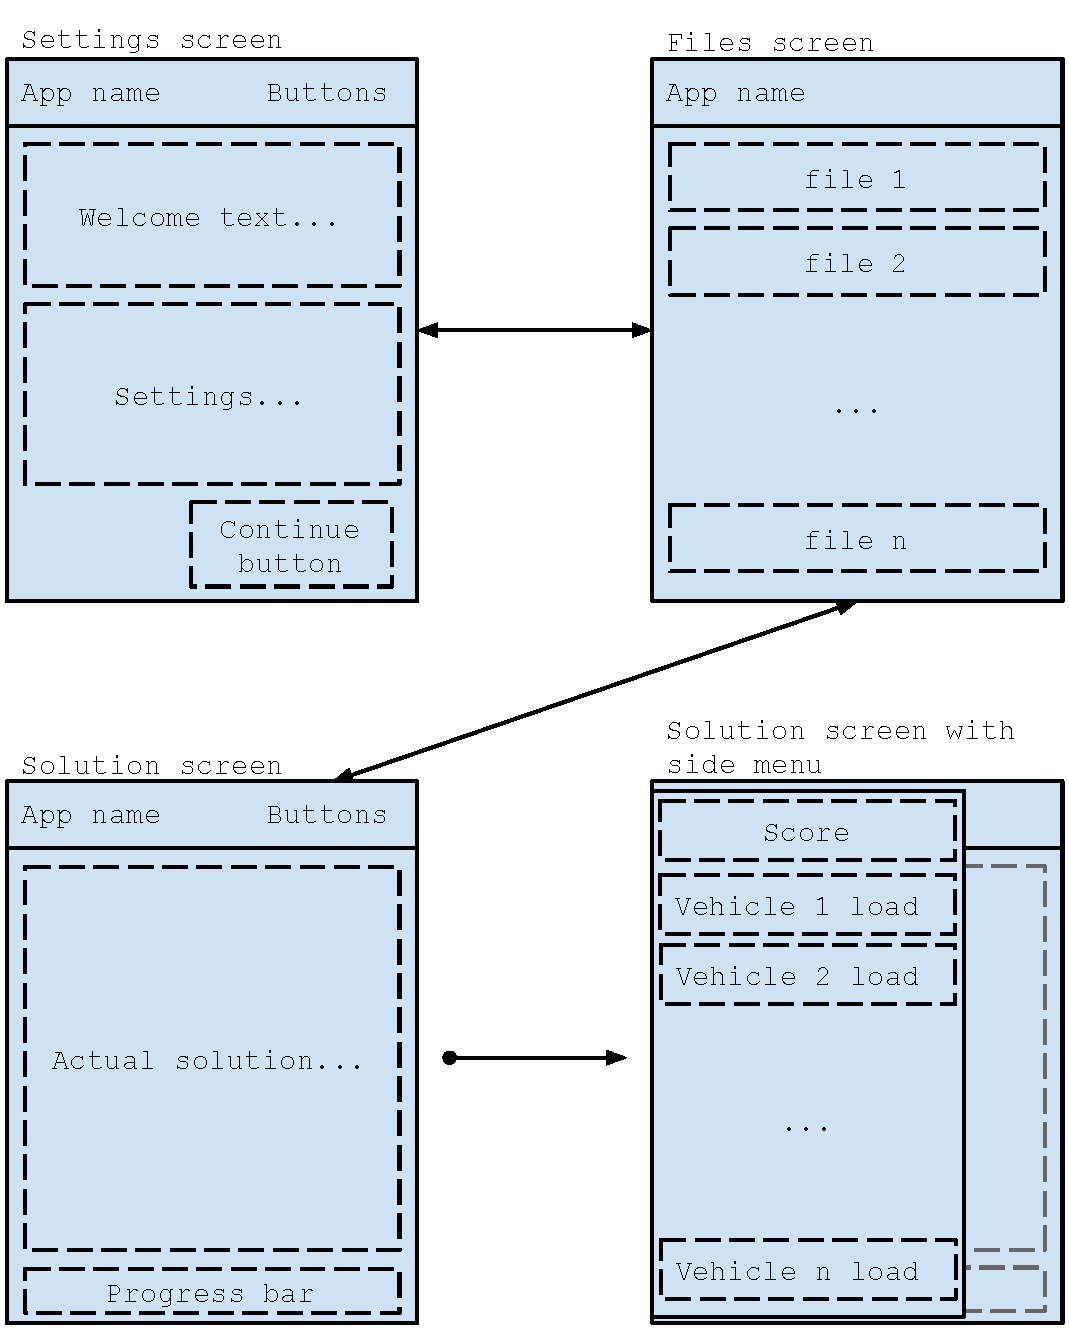
\includegraphics[scale=0.8]{fig/proposal.pdf}
    \caption{Proposal of screens}
    \label{proposalFig}
\end{figure}

\paragraph{Informational dialogs}
Application will contains two informational dialogs to better understanding application content. First one will contain
information about application itself. Second one will consist from legend which describes all displayed components of
Vehicle routing problem on the screen.

\paragraph{Material design}
One of the new features which bring Android version 5 is material design. It is very sophisticated study that show how
to handle with with elements, layouts, colors and more. Although this property is not fully backward compatible, it is
possible partially to bring this design to earlier devices with older versions of Android. This application uses
material design as much as possible. Every screen will contains material design elements which are described bellow.

\section{Application implementation}
%todo introduction to section

\subsection{Application structure} % describe inner structure not ui
Application consists from three screens. First screen is displayed after start of the application and it is used for
settings of calculation time limit and algorithm. These parameters are packed in bundle and passed to next screen after
user clicks on the Open file button placed on this screen. Second screen consist of list of example vrp files which is
provided by RecyclerView component. User selects one of the files and its name is passed to last screen together with
parameters from the first one. According to name, vrp file is open on the last screen and after click on start button
asynchronous process for calculation is created. More details about individual components are described below.

\subsubsection{Activities and fragments}
Initialy, all the application screens was implemented as activities. However, it turns out that activities have problems
with data storing and after some change of configuration (for example rotation of screen or restoring application from
background) destroyes background process and totally recreates activity. Thus framgments were used instead.

Fragments represents part of an Activity. Activity can contain multiple fragments and they can be replaced with another
fragments. They can be presented as modular section of an activity with own lifecycle.

Figure \ref{activityFragment} shows usage of fragments and activities in this application. Only one activity is presented and it
contains action bar and place for fragments. Compared to activites, only part for fragment changes and if new screen is
required this part is replaced with another fragment. Activity is recreated only in case when application is restarted
or configuration is changed.

For proper storage of state in fragment \texttt{setRetainInstance(true);} has to be called in method \texttt{onCreate()}
of current fragment.

\begin{figure}[h!]
    \centering
    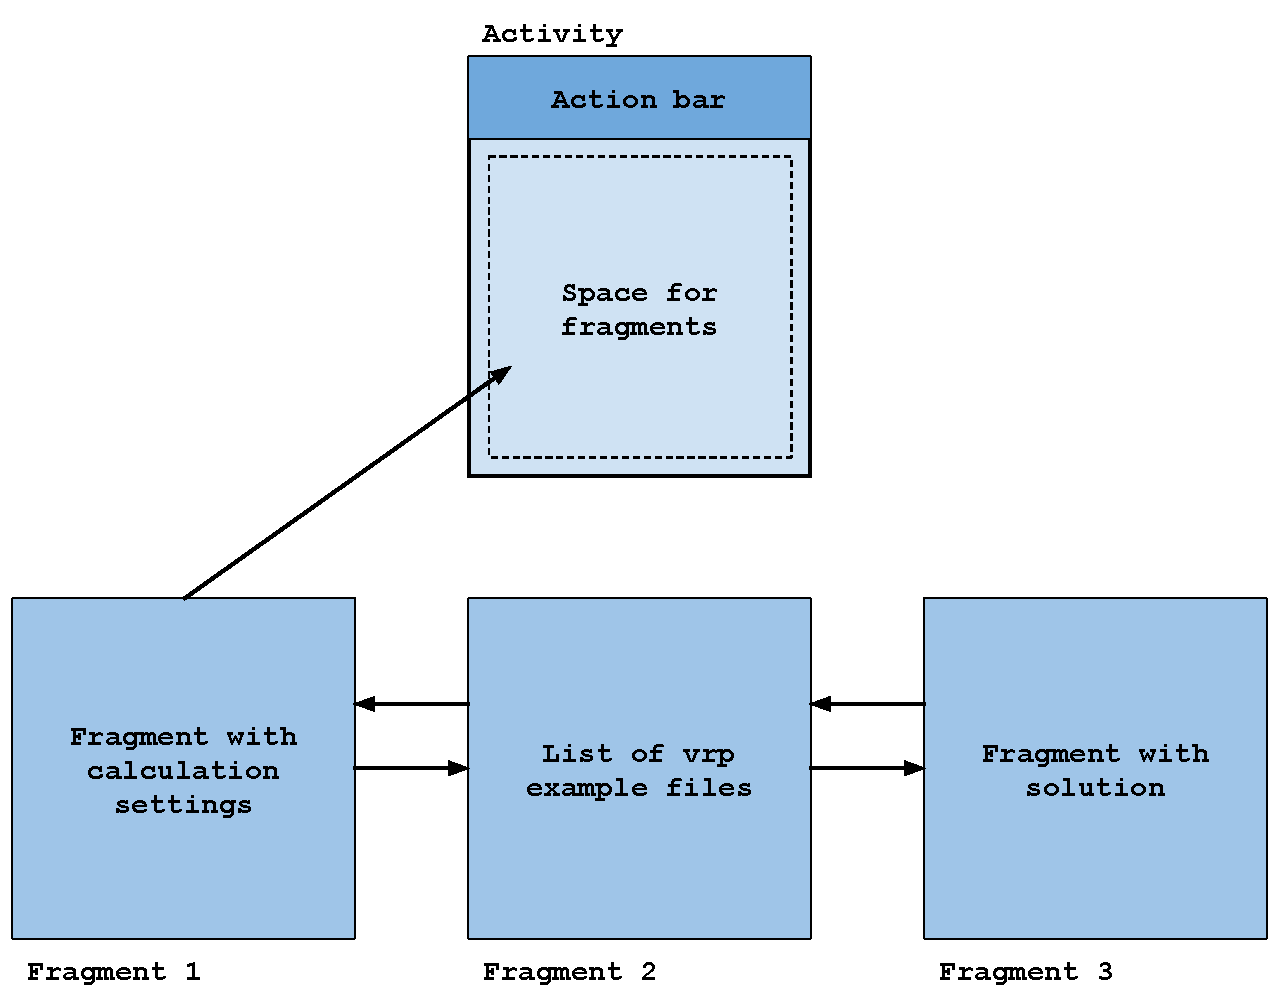
\includegraphics[scale=0.7]{fig/act_frag.pdf}
    \caption{Activity and fragments in application}
    \label{activityFragment}
\end{figure}

\subsubsection{Fragment components}
In following section, important component of application is described. Especially, these components are related to
background process and not graphical layout of application which is described in Section \ref{guiSection}.

\paragraph{List of files}
Second screen consist mainly from list of vrp example files. This list is implemented by \texttt{RecyclerView}
component. This component simplifies data displaying to list and provides basic patterns of behavior.

\paragraph{Solver asynchronous process}
After button for calculation start is pressed, asynchronous process is created. This process sets, build and run solver
with required parameters. Listener is added to solver to publish process every time when new best solution is found.
Asynchronous process is represented by \texttt{VrpSolverTask} class which extends \texttt{AsyncTask}. \texttt{AsyncTask}
class enables changes of gui, perform background operations and publishing results.

\paragraph{Solution painter}
When file is selected from list in second screen unsolved solution is painted. After start of caculation, every time
when new best solution is found solution painter draws it. Solution painter is represented by \texttt{VrpPainter} class
and it is partially modified \texttt{VehicleRoutingSolutionPainter} class from Optaplanner project. Because Android
does not support awt and swing graphic libraries, it was rewritten to use android tools. Also some other changes was
done like new appearance of customers, material design colors and more.

\subsection{Porting of Vehicle Routing Problem}
%todo introduction to subsection

\paragraph{Vehicle Routing Problem definition}
Without defining of the problem, application cannot work. Vehicle routing problem is defined by
\texttt{VehicleRoutingSolution} class which implements \texttt{Solution} interface. This class contains all information
about solved problem (list of all customers, depots and vehicles) and Solver use it together with solver configuration
to solve the problem. \texttt{Customer} class is marked as planned entity which contains \texttt{Standstill} planning
variable. More information about Vehicle Routing Problem definition can be found in OptaPlanner documentation
\cite{OptaPlannerDoc}.

\paragraph{Solver configurations}
In this application, it is possible to use three algorithms and set time limit of calculation. These configurations
including problem definition abd score calculator are stored in xml file from which is Solver built. For each algorithm
is created such file and it is selected according to the choice. Time limit is additionally set after Solver is created.

\paragraph{Score calculator}
Every solution has own score and this score must be calculated one of the three methods described in Section
\ref{scoreConfigSection}. For score calculation in this application, \texttt{VehicleRoutingEasyScoreCalculator} class
which implements \texttt{EasyScoreCalculator} is used. This class calculates hard and soft score of solution. Hard score
is computed as load of cars above their capacity. Soft score is calculated as total distance of cars. In case of time
window variant, delay against due time of arrival is added to hard score.

\paragraph{Vrp example files}
Example .vrp files are used for problem datasets. These files are taken from Vehicle Routing problem part of original
Optaplanner application. They cointains informations about number and capacity of vehicles, position and demand of
customers and position of depot. This application includes 36 example files in total.

\paragraph{Vehicle routing importer}
Example files are stored in specific vrp text format and have to be transformed into Vehicle routing solution. For this
purpose, \texttt{VehicleRoutingImporter} class is imported and used from original Optaplanner application.

\section{Graphical user interface}\label{guiSection}
%todo introduction to section

\subsection{Application screens}
Every application consists of fragments or activities which are collectively called screens. Using controls, it is
possible to move from one screen to another or change its appearance or behavior. This application is composed from
three screens. These screens can be seen in Figure \ref{screens}. The third screen is displayed with unsolved and with
solved solution.

\paragraph{Main screen}
Main screen is displayed after the application is started. It consists from action bar, welcome text, setting elements
and button to continue to another screen. Action bar contains application name and buttons for displaying legend and
application informations dialogs. Welcome text provides some basic instruction for the user. Two controls are present
for calculation options of the problem. It is possible to set time limit in seconds using Number picker and Spinner
allows select one of the three supported algorithms. Last element on this screen is Open file button which opens screen
with list of vrp files.

\paragraph{Screen with vrp files list} After Open file button from main screen is pressed this screen is displayed. It
also contains action bar but it is very litimed because no controls are required there. Basically, whole screen is
filled with list of vrp files. These example files were used from OptaPlanner project \cite{OptaPlannerPages}. After
pressing the selected file it is switched to last screen which displays problem and its solution.

\paragraph{Screen of solution}
This screen is used to displaying unsolved and solved solution. It contains action bar with all items as shown in Figure
\ref{actionBar}. Compared to the main screen, action bar has additionally button for displaying Navigation drawer and
button for start and end of the solution process. On the bottom of the screen, Progress bar is placed. This component
is used for displaying approximate remaining time. Rest of screen is filled with component which draws current solution.
This component draws unsolved solution at the beginning and after start button is pressed it draws best solution after
solver finds some. Individual elements represents:

\begin{itemize}
  \item \textbf{Circle with a number} -- customer with his demand
  \item \textbf{Building image} -- depot from which depart vehicles
  \item \textbf{Car image} -- vehicle with its color
  \item \textbf{Solid line} -- vehicle road to customer
  \item \textbf{Dashed line} -- vehicle road to depot
  \item \textbf{Sector on a circle} -- time windows for vehicle arrival
  \item \textbf{Line on a circle} -- vehicle arrival time
\end{itemize}


\begin{figure}[h!]
    \centering
    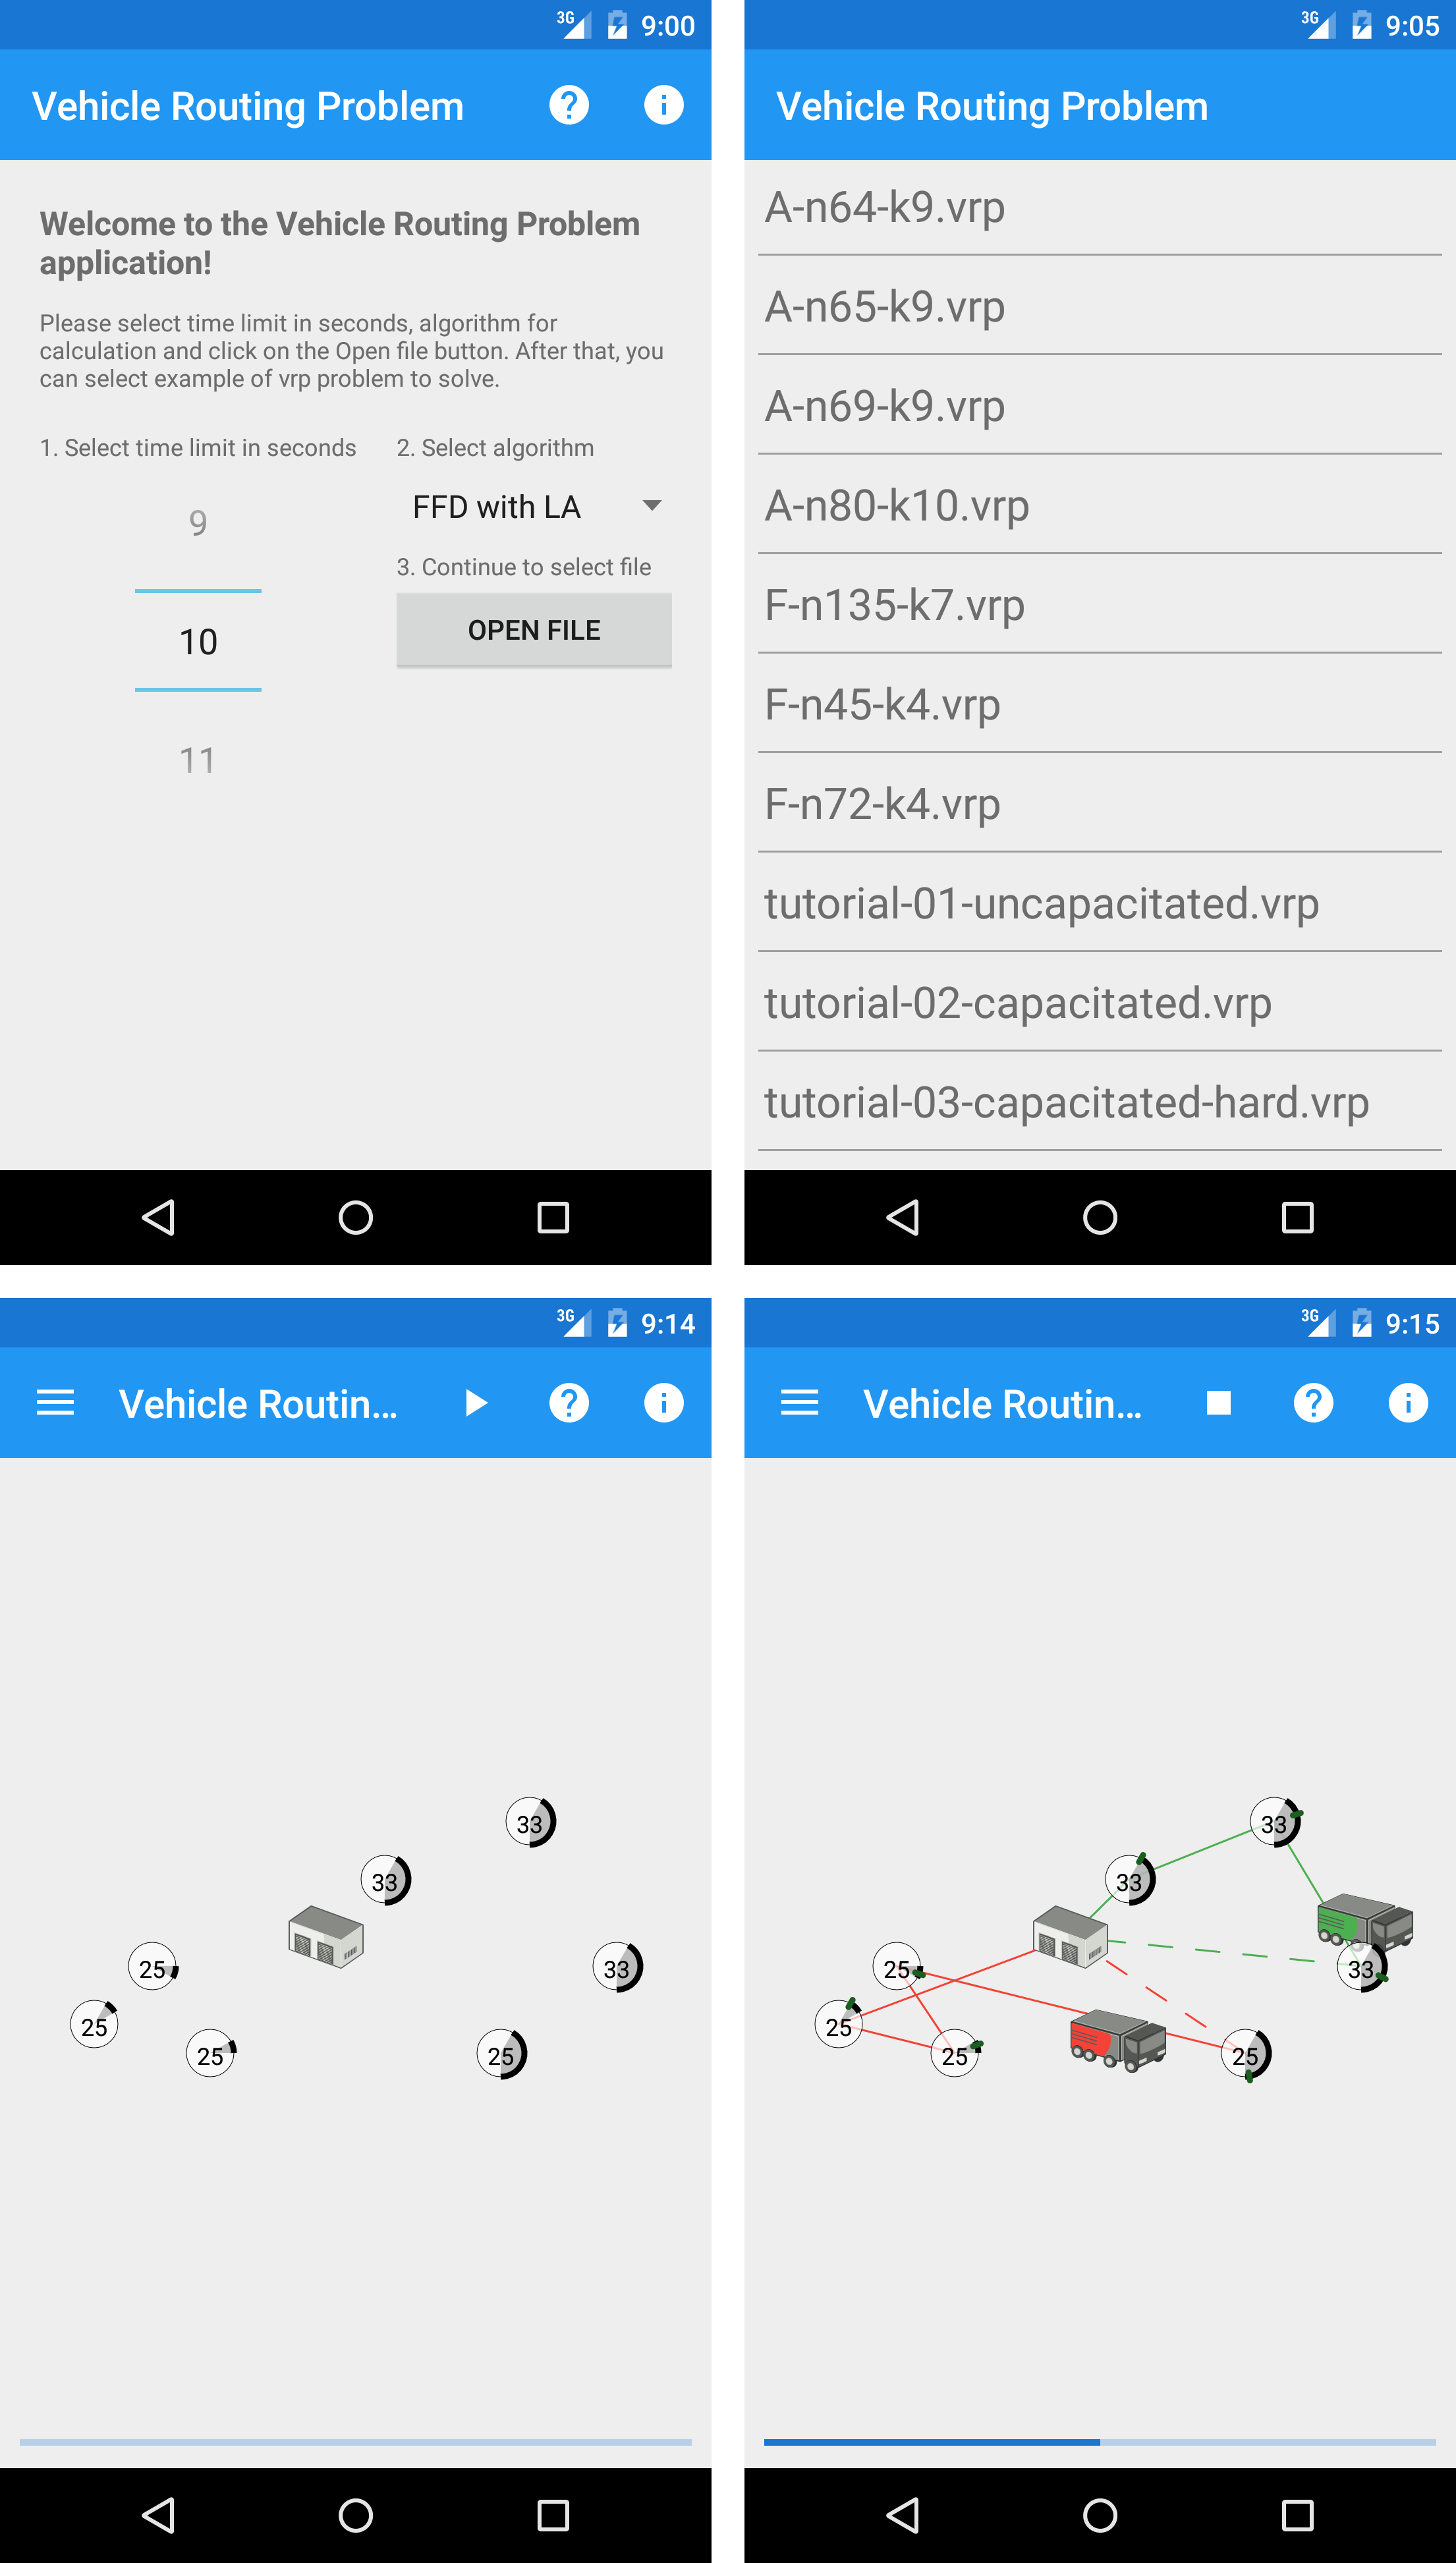
\includegraphics[scale=0.15]{fig/screens.png}
    \caption{Application screens -- main screen, list of vrp files, screen with unsolved and solved solution}
    \label{screens}
\end{figure}

\subsection{Application components}
%todo introduction to subsection

\subsubsection{Action bar}
Action bar is a panel on top of the screen that provides basic user action and informations about user navigation. It
always contains application name, optionally actions buttons for quick invocation of application functionalit and
overflow button on the right side for diplaying other applications options.

Action bar is diplayed on every screen of this application but it changes depending on required functions on actual
screen. Figure \ref{actionBar} show action bar of screen where solved problems are shown. The panel contains buttons for
displaying of navigation drawer and dialogs which are described below and application name.

\begin{figure}[h!]
    \centering
    
\includegraphics[scale=0.15]{fig/action_bar.png}
    \caption{Action bar}
    \label{actionBar}
\end{figure}

\subsubsection{Navigation drawer}
Navigation drawer is a panel that displays application navigation on the left edge of the screen. By default, it is
hidden and it could be displayed by touch the left icon on the action bar. Also it could be displayed whe a user swipes
with a finger from the left edge of the screen to the right. Opposite procedure makes navigation drawer invisible.

This application uses navigation drawer for displaying important computing data. Figure \ref{navigationDrawer} displays
visible panel on the left side of the application. First item shows hard and soft score of currently the best solution
found. Second item holds total distance of all cars. Other items are linked to cars of the problem. Every car has own
parameters -- color, name and capacity. These three are static and do not change during the calculation. Last parametr
is actual load of the vehicle.

\begin{figure}[h!]
    \centering
    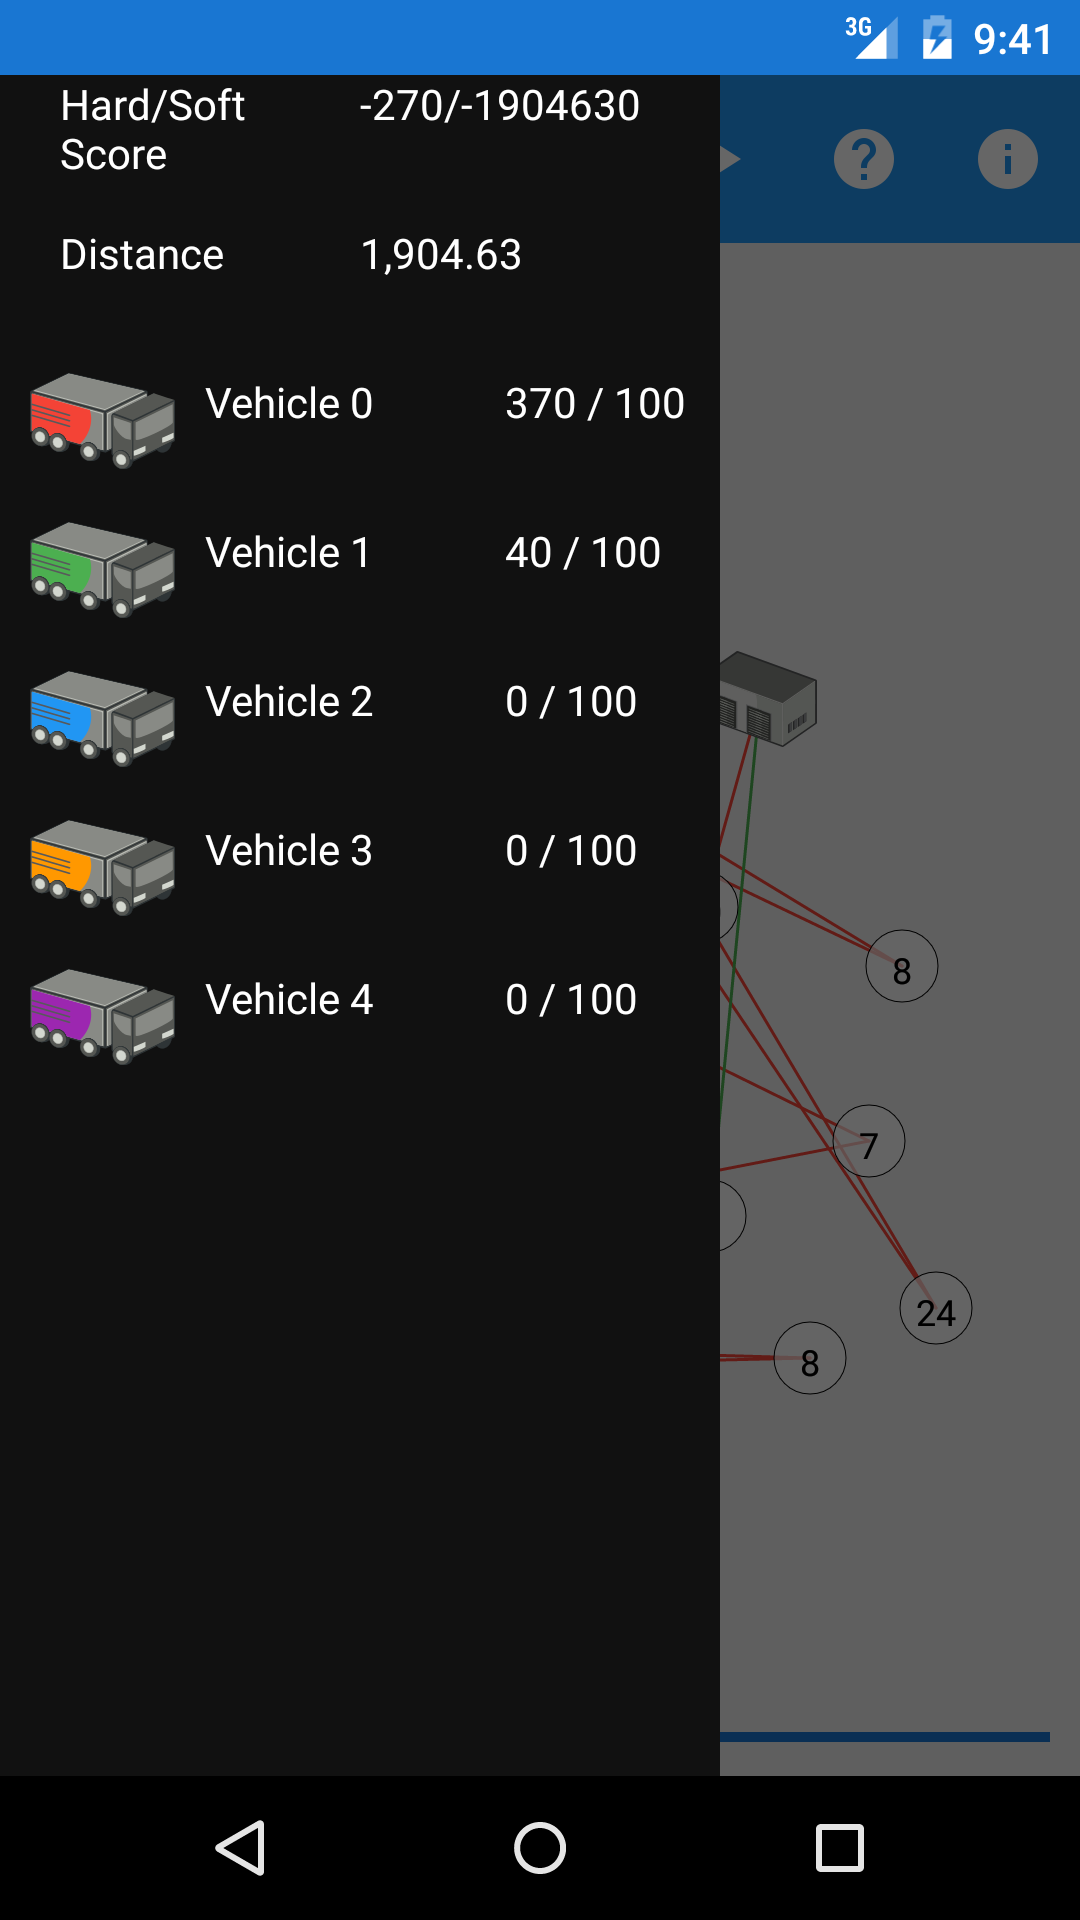
\includegraphics[scale=0.15]{fig/nav_drawer.png}
    \caption{Navigation drawer with actual data}
    \label{navigationDrawer}
\end{figure}

\subsubsection{Dialogs}
Dialogs are small windows which displays some significant informations or are used for user interaction with a decision
that decides on further actions. Dialogs are always located above all other parts of the application

Figure \ref{dialogs} shows all three dialogs which are used in the application. Two of them can be retrieved directly from the
action bar by clicking on the icon with a question mark or the informative icon. First dialog contains application
legend for understanding what is displayed on the screen and second dialog briefly describes the application. Third
dialog is displayed only solving is running and user clicks on the back button. Dialog asks the user if he wants to end
the ongoing calculation.

\begin{figure}[h!]
    \centering
    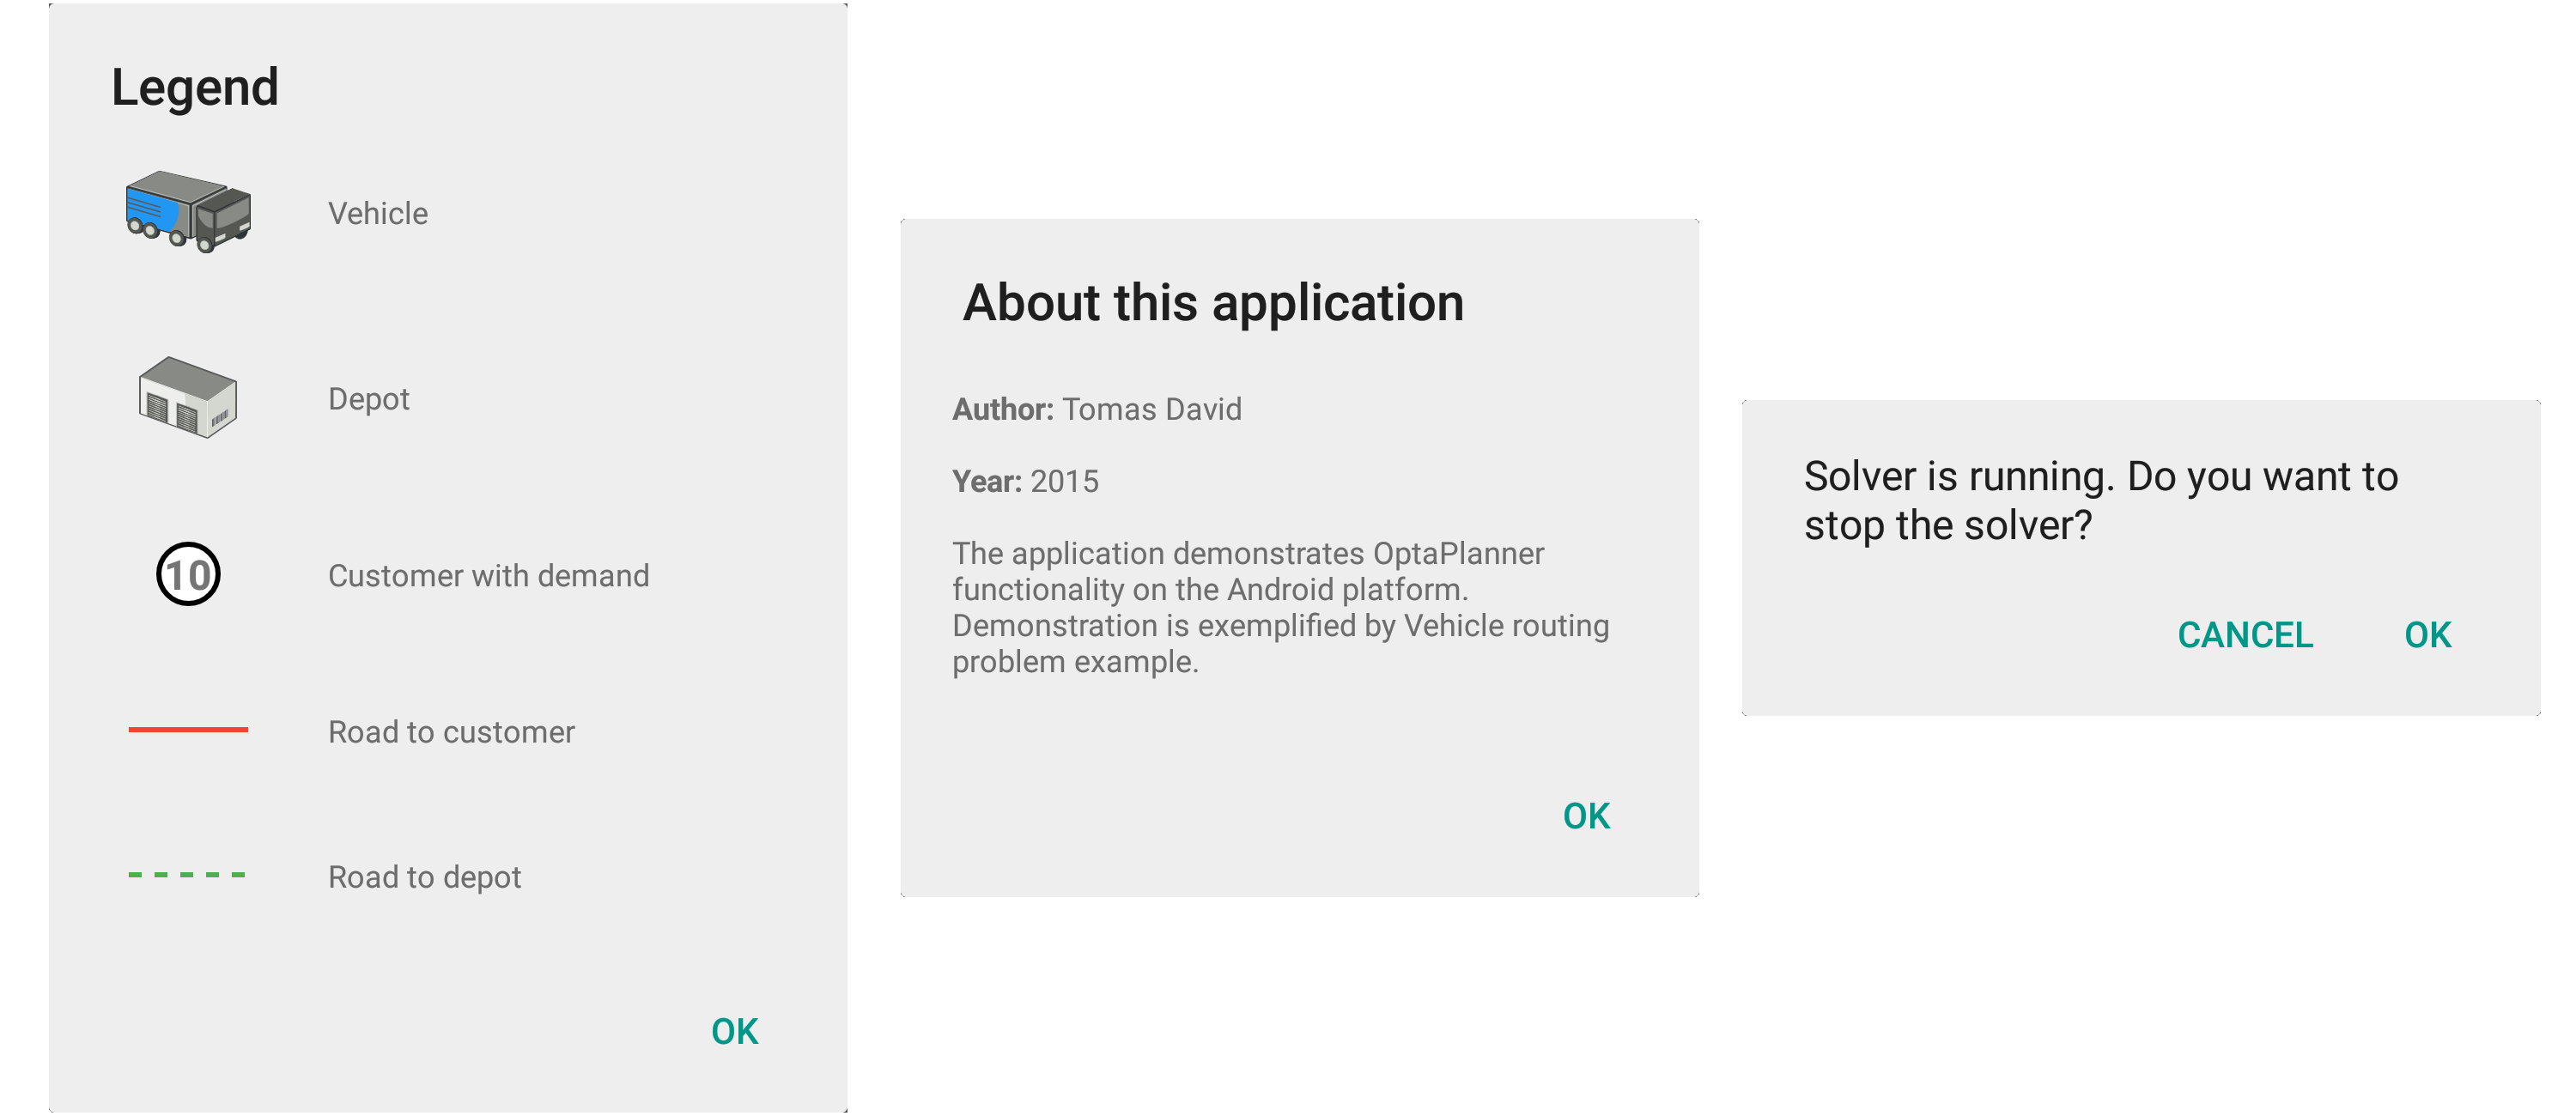
\includegraphics[scale=0.15]{fig/dialogs.png}
    \caption{dialogs used in the application}
    \label{dialogs}
\end{figure}
